\section{Experimental Results}\label{sec:experiments}

In this section we effectuate a comparison between the different extractors provided by the PCA and the LDA in association with the different techniques  of components selection. We organized our experiments focusing on a given adversary, whose aim is to optimally choose an extraction method with respect to the four criteria described in Appendix ~\ref{sec:fourCriteria}. Thus, we consider four scenarios: in each one, three of the four parameters $\numTraces[], \numTraces[]', \newTraceLength, \numPoI$ are fixed and one varies. For those in which $\numTraces[]'$ is fixed, the value of $\numTraces[]'$ is chosen high enough to avoid the SSS problem; then, the extensions of LDA presented in Sec.~\ref{sec:SSS} are not evaluated.\footnote{This study is let open for an extended version of this paper.} As a consequence, for these three scenarios, we always perform the LDA in a favourable situation, which makes expect the LDA to be more efficient than the PCA in our experiments. Our goal is therefore only to study whether the PCA can be made almost as efficient than the LDA thanks to the component selection methods discussed in Sec.~\ref{sec:ELV}. 



\subsubsection{The testing adversary.}  Our testing adversary attacks an 8-bit AVR microprocessor Atmega328P and acquires power-consumption traces via the ChipWhispered platform \cite{o2014chipwhisperer}.\footnote{This choice has been done, in particular, to allow for reproducibility of the experiments.} The target device stores a secret 128-bits key and performs the first steps of an AES: the reading of 16 bytes of the plaintext, the AddRoundKey step and the AES Sbox. It has been programmed twice: two different keys are stored in the device memory during the acquisition of the profiling and of the attack traces, to simulate the situation of two identical devices storing a different secret. The size of the traces equals $\traceLength = 3996$. The target sensitive variable is the output of the first Sbox byte, but, since the key is fixed also during the profiling phase, and both Xor and Sbox operations are bijective, we expect to detect three interesting regions: the reading of the first byte of the plaintext, the first AddRoundKey and the first Sbox. We consider an {\em identity classification} leaking function (i.e. we make minimal assumption on the leakage function), which implies that the 256 possible values of the Sbox output gives birth to 256 classes. For each class we assume that the adversary acquires the same number $N_p$ of traces, \textit{i.e.} $\numTraces[]' = N_p\times 256$. After the application of the extractor $\extract$, the trace size is reduced to $\newTraceLength$. Then the attacker performs a Bayesian Template Attack \cite{Chari2003}, using $\newTraceLength$-variate Gaussian templates.
\begin{figure}[h!]
\subfigure[]{\label{fig:1.1}
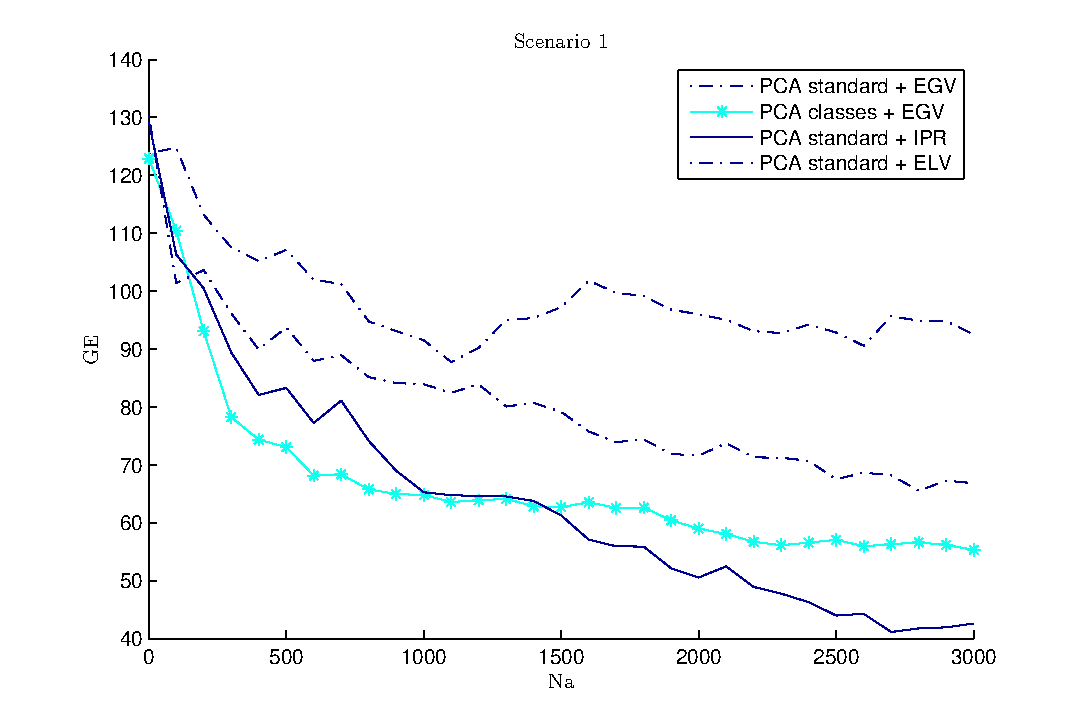
\includegraphics[width=0.5\textwidth]{figures/Criterion1.pdf}}
\subfigure[]{\label{fig:1.2}
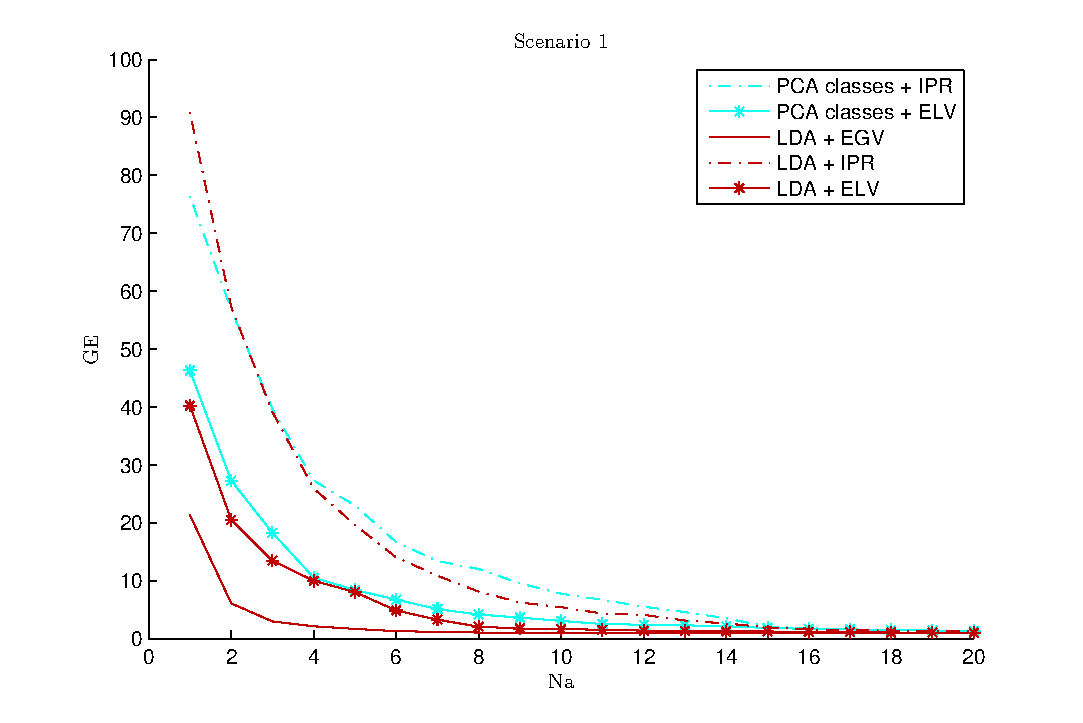
\includegraphics[width=0.5\textwidth]{figures/Criterion1Good.pdf}}
\subfigure[]{\label{fig:2.1}
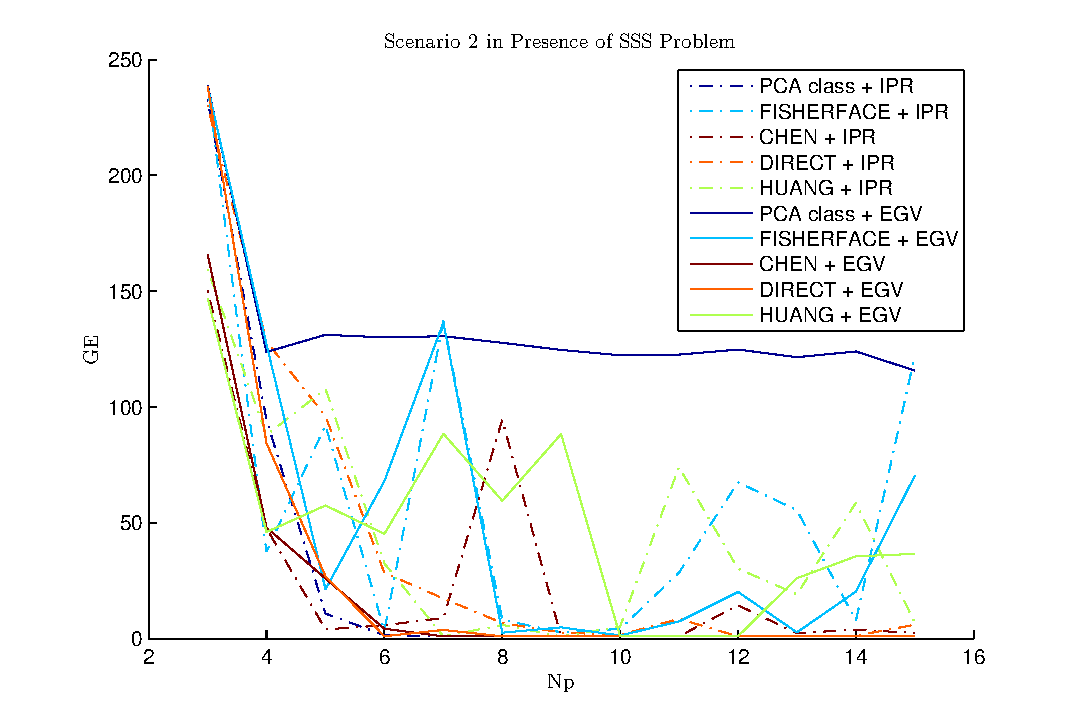
\includegraphics[width=0.5\textwidth]{figures/Criterion2SSS.pdf}}
\subfigure[]{\label{fig:2.2}
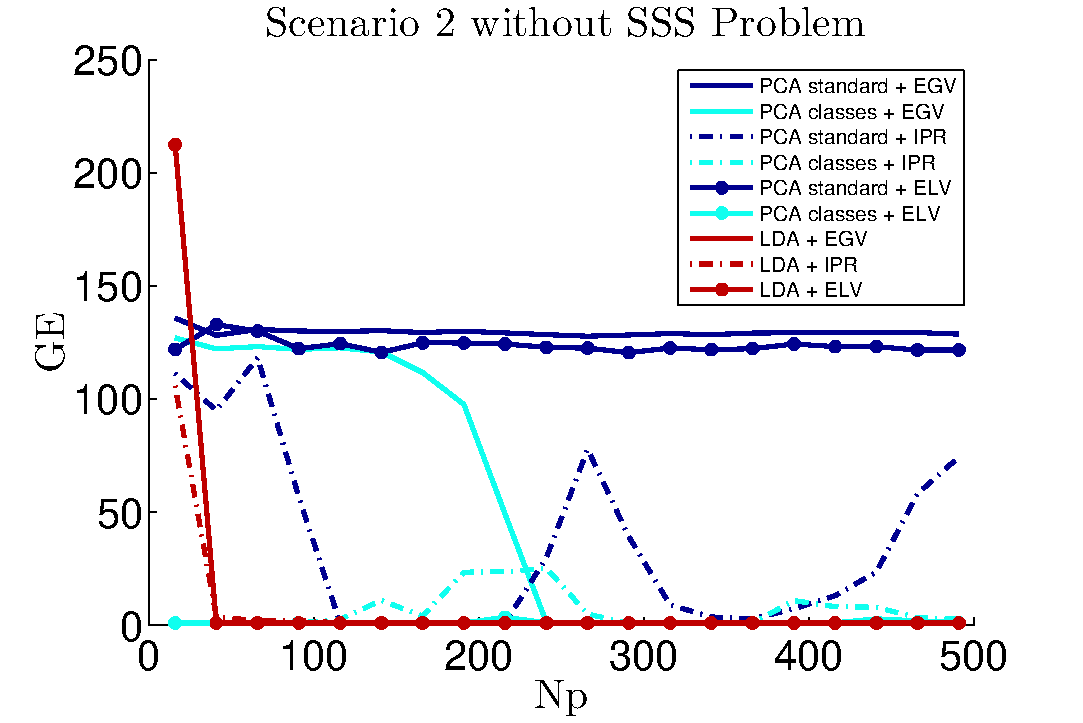
\includegraphics[width=0.5\textwidth]{figures/Criterion2notSSS.pdf}}
\caption{Guessing Entropy as function of the number of attack traces \ref{fig:1.1},\ref{fig:1.2} and of the number of profiling traces per class \ref{fig:2.1}, \ref{fig:2.2}, for different extraction methods. In \ref{fig:2.1} the LDA is substituted by its extensions to handle the SSS problem. All Guessing Entropies are estimated as the average rank of the right key over 100 independent experiments.}\label{fig:1and2}
\end{figure}


\subsubsection{Scenario 1.}
To analyse the dependence between our extraction methods, presented in Sec.~\ref{sec:ELV}, and the number of attack traces $\numTraces[]$ needed to achieve a given GE, we fixed the other parameters as follows: $N_p=50$ ($\numTraces[]'=50*256$), $\newTraceLength = 3$ and $\numPoI = 3996$ (all points are allowed to participate in the building of PCs and LDCs). The experimental results, depicted in Fig.~\ref{fig:1and2} \subref{fig:1.1}-\subref{fig:1.2}, show that the PCA standard method has very bad performances in SCA, while the LDA is the method that performs best. Concerning the class-oriented PCA, we observe that its performance its comparable to that of LDA, when combined with the selection methods ELV (which performs best) or IPR.  


\subsubsection{Scenario 2.}
%\begin{figure}
%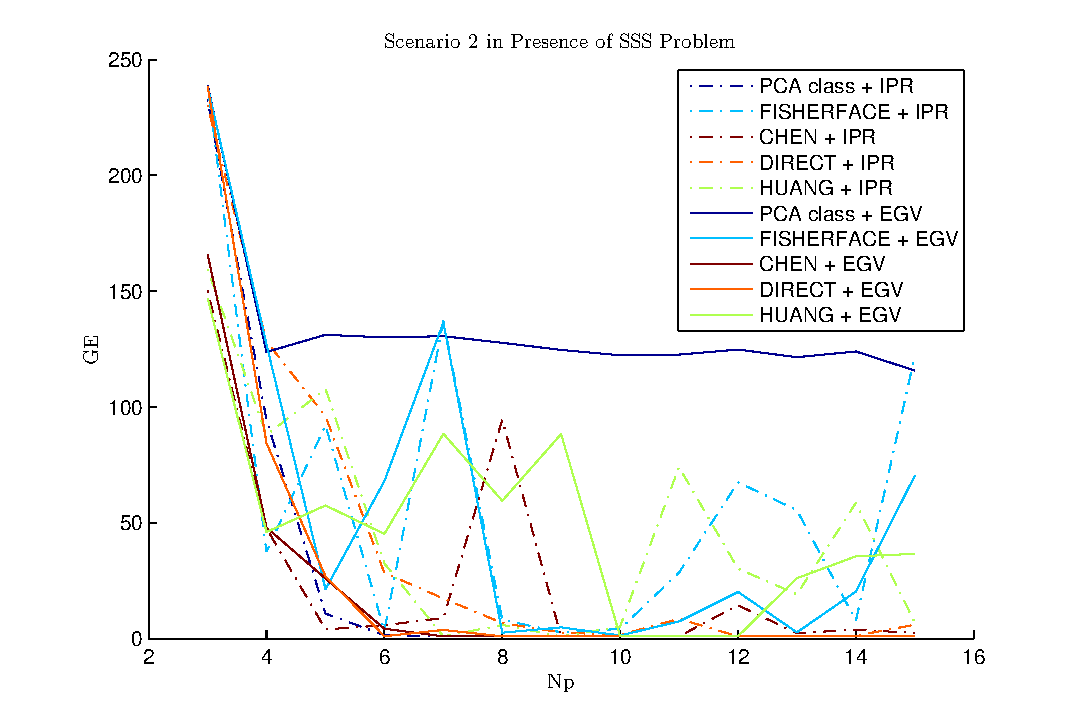
\includegraphics[width=0.5\textwidth]{figures/Criterion2SSS.pdf}
%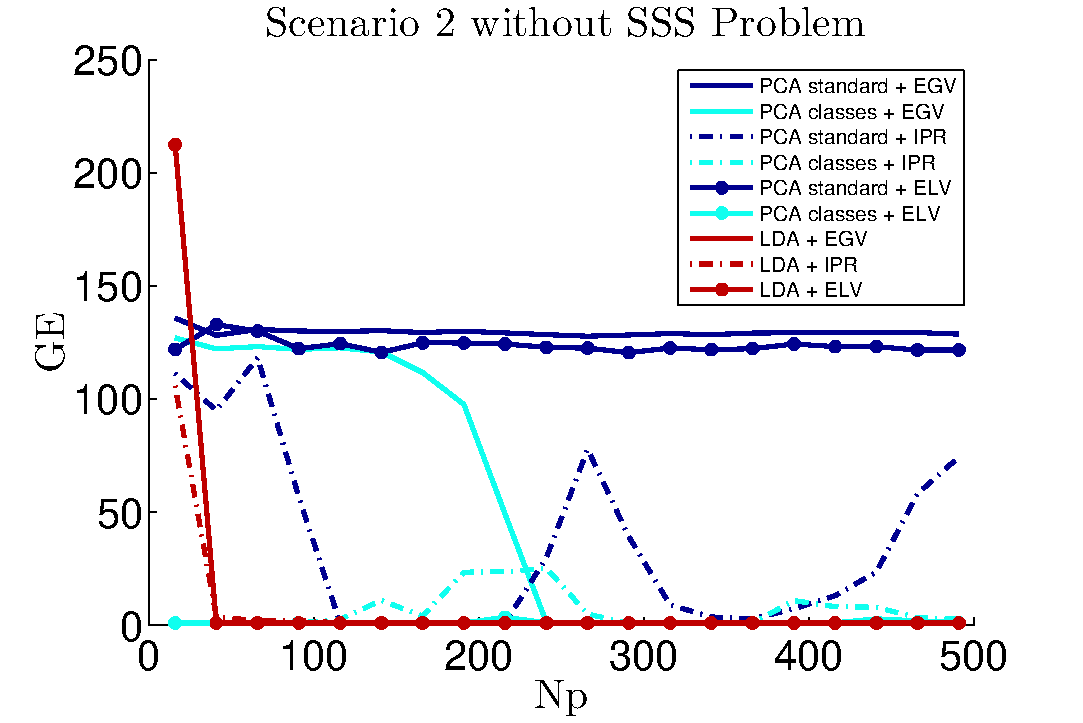
\includegraphics[width=0.5\textwidth]{figures/Criterion2notSSS.pdf} 
%\caption{Guessing Entropy as function of the number of profiling traces per class, for different extraction methods: on the left the LDA is substituted by its extensions to handle the SSS problem.}\label{fig:2}
%\end{figure}
Now we test the behaviour of the extraction methods, as function of the number $N_p$ of available profiling traces per class. The number of components $\newTraceLength$ is still fixed to 3, and $\numPoI=3996$ again. This scenario has to be divided into two parts: if $N_p\leq 15$, then $\numTraces[]'<\traceLength$ and the SSS problem occurs. Thus, in this case we will test the four extensions of LDA presented in Sec.~\ref{sec:SSS}, associated to either the standard selection, to which we abusively refer as EGV,\footnote{It consists in keeping the $\newTraceLength$ first LDCs, except for the Direct LDA, which asks to keep the last LDCs.} and to the IPR selection.  We compare them to the class-oriented PCA associated to the same selection methods. The ELV selection is not performed in this case because, for some of the techniques extending LDA, the projecting LDCs are not associated to some eigenvalues in a meaningful way. On the contrary, if $N_p\geq 16$ there is no need to approximate the LDA technique, so the classical one is performed. Results for this scenario are shown in Fig.~\ref{fig:1and2} \subref{fig:2.1}-\subref{fig:2.2}. It may be noticed that the combination class-oriented PCA + IPR does not suffer the lack of profiling traces; anyway, it is outperformed by the Chen method in association to EGV. The Direct LDA method also provides a good alternative, while the other tested methods do not show a stable behaviour. The results in absence of the SSS problem confirm that the standard PCA is not adapted to SCA, even when provided with more profiling traces. It also shows that among class-oriented PCA and LDA, the class-oriented PCA converges faster.



\medskip

  \begin{minipage}[c]{\textwidth}
  \hspace*{-3mm}
  \begin{minipage}[c]{0.49\textwidth}
    \centering
    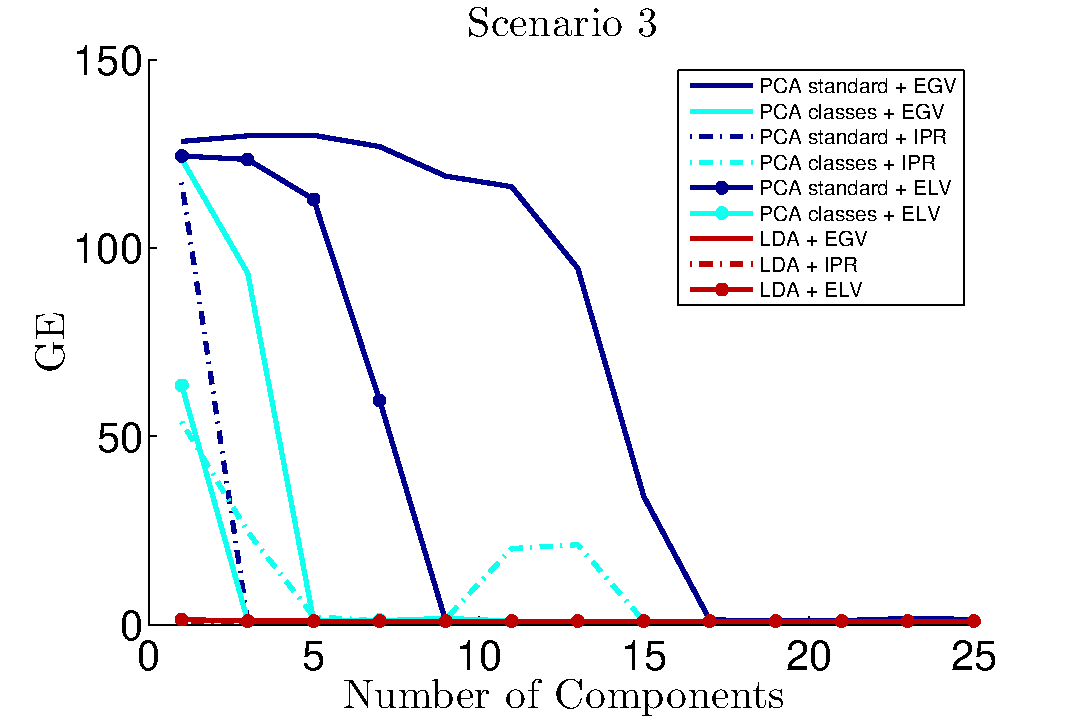
\includegraphics[width=\textwidth]{figures/Criterion3.pdf}
    \captionof{figure}{Guessing Entropy as function of the number of the traces size after reduction}\label{fig:3}
  \end{minipage}
\hspace{1mm}
  \begin{minipage}[c]{0.45\textwidth}
    \centering
    \begin{tiny}
\begin{tabular}{|c|c|c|c|c|c|}
\hline
&&\multicolumn{4}{|>{\columncolor[gray]{0.7}}c|}{Parameter to minimize}\\
\hline
\multicolumn{1}{|>{\columncolor[gray]{0.7}}c|}{Method}&\multicolumn{1}{|>{\columncolor[gray]{0.7}}c|}{Selection}& $N$ &  $N'$ (SSS) &  $N'$ (not SSS) &  $C$ \\
\hline
PCA standard & EGV & {\bf -} &  &{\bf -} &{\bf -} \\
\hline
PCA standard &\multicolumn{1}{|>{\columncolor[gray]{0.8}}c|}{ELV} & \multicolumn{1}{|>{\columncolor[gray]{0.9}}c|}{{\bf -}} & &\multicolumn{1}{|>{\columncolor[gray]{0.9}}c|}{{\bf -}} &\multicolumn{1}{|>{\columncolor[gray]{0.9}}c|}{{\bf -}} \\
\hline
PCA standard & IPR &{\bf -} & &{\bf -} &{\bf +} \\
\hline
PCA class & EGV & {\bf -} &{\bf -} &{\bf -} &{\bf -} \\
\hline
PCA class & \multicolumn{1}{|>{\columncolor[gray]{0.8}}c|}{ELV} &\multicolumn{1}{|>{\columncolor[gray]{0.9}}c|}{{\bf +}} & &\multicolumn{1}{|>{\columncolor[gray]{0.9}}c|}{$\bigstar$} &\multicolumn{1}{|>{\columncolor[gray]{0.9}}c|}{{\bf +}} \\
\hline 
PCA class & IPR & {\bf {\bf +}} &$\bigstar$ &{\bf +} &{\bf -} \\
\hline 
LDA & EGV &$\bigstar$ & & {\bf +} & $\bigstar$\\
\hline 
LDA & \multicolumn{1}{|>{\columncolor[gray]{0.8}}c|}{ELV} & \multicolumn{1}{|>{\columncolor[gray]{0.9}}c|}{{\bf +}} &  & \multicolumn{1}{|>{\columncolor[gray]{0.9}}c|}{{\bf +}} & \multicolumn{1}{|>{\columncolor[gray]{0.9}}c|}{$\bigstar$}\\
\hline 
LDA & IPR & {\bf +} & &{\bf +} & $\bigstar$ \\

\hline 
\multicolumn{1}{|>{\columncolor[gray]{0.8}}c|}{Chen}  & EGV & &\multicolumn{1}{|>{\columncolor[gray]{0.9}}c|}{$\bigstar$ } & & \\
\hline 
\multicolumn{1}{|>{\columncolor[gray]{0.8}}c|}{Chen}  & IPR & &\multicolumn{1}{|>{\columncolor[gray]{0.9}}c|}{{\bf +}} & & \\
\hline 
\multicolumn{1}{|>{\columncolor[gray]{0.8}}c|}{Direct LDA} & EGV & & \multicolumn{1}{|>{\columncolor[gray]{0.9}}c|}{$\bigstar$}& & \\
\hline 
\multicolumn{1}{|>{\columncolor[gray]{0.8}}c|}{Direct LDA} & IPR & &\multicolumn{1}{|>{\columncolor[gray]{0.9}}c|}{{\bf +}}& & \\
\hline
\multicolumn{2}{|>{\columncolor[gray]{0.8}}c|}{Fisherface} & &\multicolumn{1}{|>{\columncolor[gray]{0.9}}c|}{{\bf -}} & & \\
\hline 
\multicolumn{2}{|>{\columncolor[gray]{0.8}}c|}{Huang}  & &\multicolumn{1}{|>{\columncolor[gray]{0.9}}c|}{{\bf -}} & & \\
\hline
\end{tabular}
\end{tiny}
\captionof{table}{Overview of extractors performances in tested situations.}\label{table:results}
    \end{minipage}
  \end{minipage}


\subsubsection{Scenario 3.}
Let  $\newTraceLength$ be now variable and let the other parameters be fixed as follows: $\numTraces[] = 100, N_p=200, \numPoI = 3996$. Looking at Fig.~\ref{fig:3}, we might observe that the standard PCA might actually well perform in SCA context if provided with a larger number of kept components; on the contrary, a little number of components suffices to the LDA. Finally, keeping more of the necessary do not worsen the efficiency of the attack, which allows adversary to choose $\newTraceLength$ as the maximum value supported by their computational means.



\subsubsection{Scenario 4.}
\begin{figure}
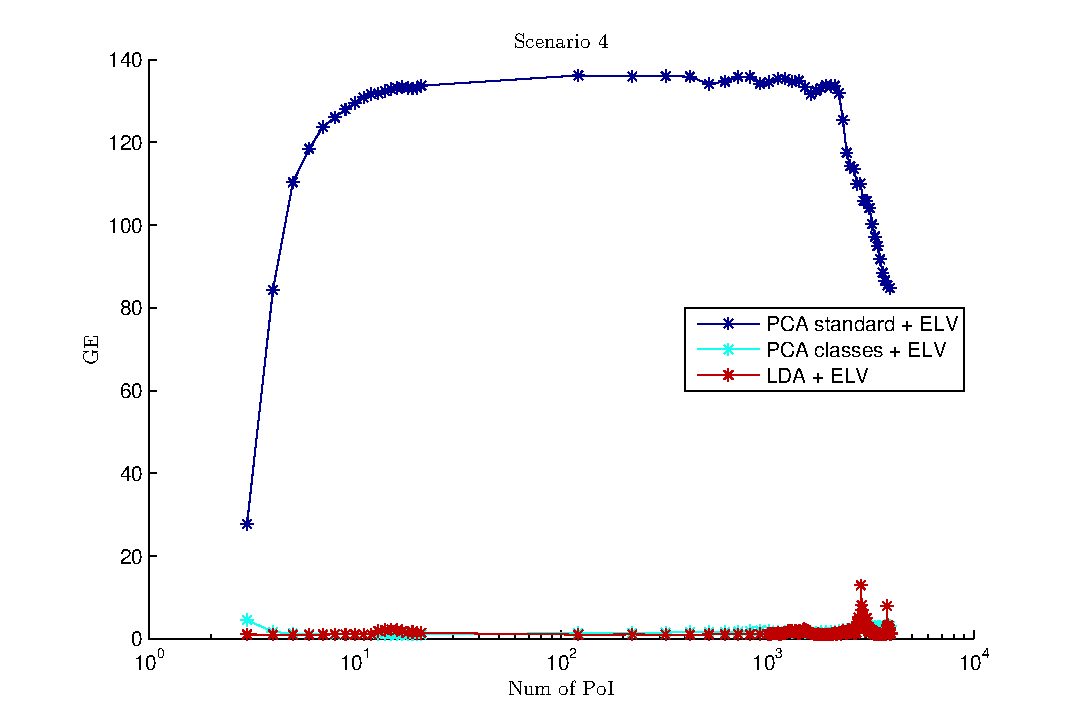
\includegraphics[width=0.5\textwidth]{figures/Criterion4.pdf}
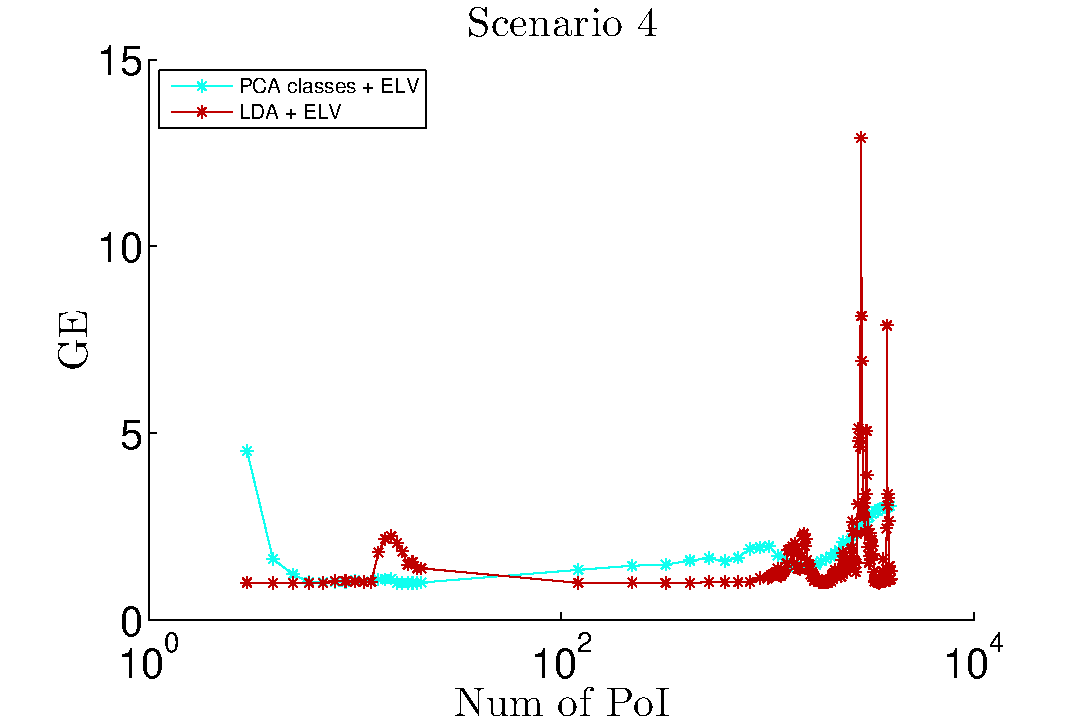
\includegraphics[width=0.5\textwidth]{figures/Criterion4cutted.pdf} 
\caption{Guessing Entropy as function of the number of time samples contributing in the extractor computation.}\label{fig:4}
\end{figure}

This is the single scenario in which we allow the ELV selection method to not only select the components to keep but also to modify them, keeping only some coefficients within each component, setting the other ones to zero. We select couples \textit{(component, time sample)} in decreasing order of the ELV values, allowing the presence of only $\newTraceLength = 3$ components and $\numPoI$ different times samples: to be clearer, we impose that the matrix $A$ defining the extractor (see \eqref{eq:linearExtractor}) has 3 rows (storing the 3 chosen components, transposed) and exactly $\numPoI$ non-zero columns.
Looking at Fig.~\ref{fig:4} we might observe that the LDA allows to achieve the maximal guessing entropy with only 1 PoI in each of the 3 selected components. 
Actually, adding PoIs worsen its performances, which is coherent with the assumption that the vulnerable information leaks in only a few points, that are excellently detected by the LDA, and that adding contribution from other points raises the noise which is then compensated by the contributions of other noisy points, in a very delicate balance. Such a behaviour is clearly visible in standard PCA case: the first 10 points considered raise the level of noise, that is then balanced by the last 1000 points.

\medskip

An overview of the results of our comparison in scenarios 1, 2 and 3 is depicted in Table\ref{table:results}: depending on the adversary purpose, given by the parameter to minimize, a $\bigstar$ denotes the best method, a ${\bf +}$ denotes a method with performances comparable to those of the best one and a ${\bf -}$ is for methods that show lower performances. Techniques introduced in this paper are highlighted by a grey background. We remark for example that the class-oriented PCA and the LDA methods take advantage by the association with our ELV selection of components and that, among the techniques that extend the LDA in presence of the SSS problem, we found out that some achieve optimal performances.



